\documentclass[11pt,a4paper]{article}

\usepackage[utf8]{inputenc}
% \usepackage[T1]{fontenc}
\usepackage[english]{babel}
\usepackage{geometry}
\usepackage{graphicx}
\usepackage{booktabs}
\usepackage{amsmath}
\usepackage{hyperref}
\usepackage{float}
\usepackage{caption}
\usepackage{subcaption}

\geometry{margin=2.5cm}

\title{Acoustic Species Identification in the Pantanal\\
\large Classical Machine Learning Approach for BirdCLEF+ 2026}
\author{Sheharyar\\
Master 1 Informatique — Sorbonne Université\\
Machine Learning Course — S2 2025--2026}
\date{May 2026}

\begin{document}

\maketitle

\begin{abstract}
This report presents a classical machine learning pipeline for identifying wildlife species from audio recordings collected in the Brazilian Pantanal, as part of the BirdCLEF+ 2026 competition. Since neural networks were not allowed, I focused on hand-crafted audio features and traditional classifiers. I extracted features like MFCCs, spectral descriptors, and chroma from around 35,500 training recordings covering 206 species with available training audio (out of 234 target species in total — 28 species only appear in the soundscape labels). I compared several models including Random Forest, Logistic Regression, LightGBM, Linear SVM, and k-NN. The best result on audio features alone was achieved by Logistic Regression with a macro ROC-AUC of 0.897 on 5-fold cross-validation; adding four non-audio metadata features (location, recording rating, source) pushed this further to 0.922. I also investigated the domain shift between clean training audio and noisy field soundscapes, and found a significant performance gap. The report covers feature engineering, model comparison, hyperparameter tuning, ablation studies, non-audio metadata, and error analysis.
\end{abstract}

% ============================================================
\section{Introduction}

Biodiversity monitoring is important for conservation, but manually identifying species from field recordings is slow and requires expert knowledge. Automated acoustic identification could help scale this effort. The BirdCLEF+ 2026 competition provides a dataset of audio recordings from the Pantanal wetlands in Brazil, covering not just birds but also amphibians, mammals, reptiles, and insects — 234 species in total.

The task is to predict which species are present in 5-second segments of field recordings. This is a multi-label problem (multiple species can be present at once), though for this project I simplified it to single-label classification. During evaluation on soundscapes, a prediction was considered correct if the predicted species was among the annotated species for that segment.

The main constraint for this project was that neural networks were not allowed. This meant I couldn't use standard approaches like CNNs on spectrograms or pretrained models like BirdNET. Instead, I had to manually design audio features and use classical machine learning methods. While this limits performance compared to deep learning, it forced me to understand what actually makes audio signals distinguishable — which is the pedagogical goal of the course.

Before running the experiments, I formulated a few working hypotheses to guide the analysis:

\begin{itemize}
    \item \textbf{H1:} MFCCs will be the dominant feature group, since they are specifically designed to capture the spectral envelope that distinguishes different sound sources.
    \item \textbf{H2:} Non-linear ensemble models (Random Forest, LightGBM) will outperform linear classifiers, given the complexity of separating 200+ classes.
    \item \textbf{H3:} A significant domain shift will exist between clean training recordings and noisy field soundscapes, causing performance to drop substantially on the latter.
\end{itemize}

These hypotheses are revisited in Section~\ref{sec:discussion}, where H1 and H3 are confirmed and H2 is falsified — a result that turned out to be one of the more interesting findings of the project.

% ============================================================
\section{Dataset}

\subsection{Overview}

The dataset consists of several components:

\begin{itemize}
    \item \textbf{train\_audio/}: 35,549 short recordings of individual species, organized in subdirectories by species label. These come from Xeno-canto and iNaturalist, all resampled to 32 kHz.
    \item \textbf{train.csv}: metadata for each recording — species label, geographic coordinates, quality rating, recording source, etc.
    \item \textbf{taxonomy.csv}: maps the 234 target species to their scientific names and taxonomic classes (Aves, Amphibia, Insecta, Mammalia, Reptilia).
    \item \textbf{train\_soundscapes/}: about 10,600 longer field recordings from the same region as the test data.
    \item \textbf{train\_soundscapes\_labels.csv}: expert-annotated labels for 1,478 five-second segments from the soundscapes.
\end{itemize}

\subsection{Class distribution}

The dataset is heavily imbalanced. The most represented species has 499 recordings, while 25 species have fewer than 10 samples and 4 species have only 1 sample each. Additionally, 28 target species (mostly insect sonotypes) have no training audio at all — they only appear in the soundscape labels.

\begin{figure}[H]
    \centering
    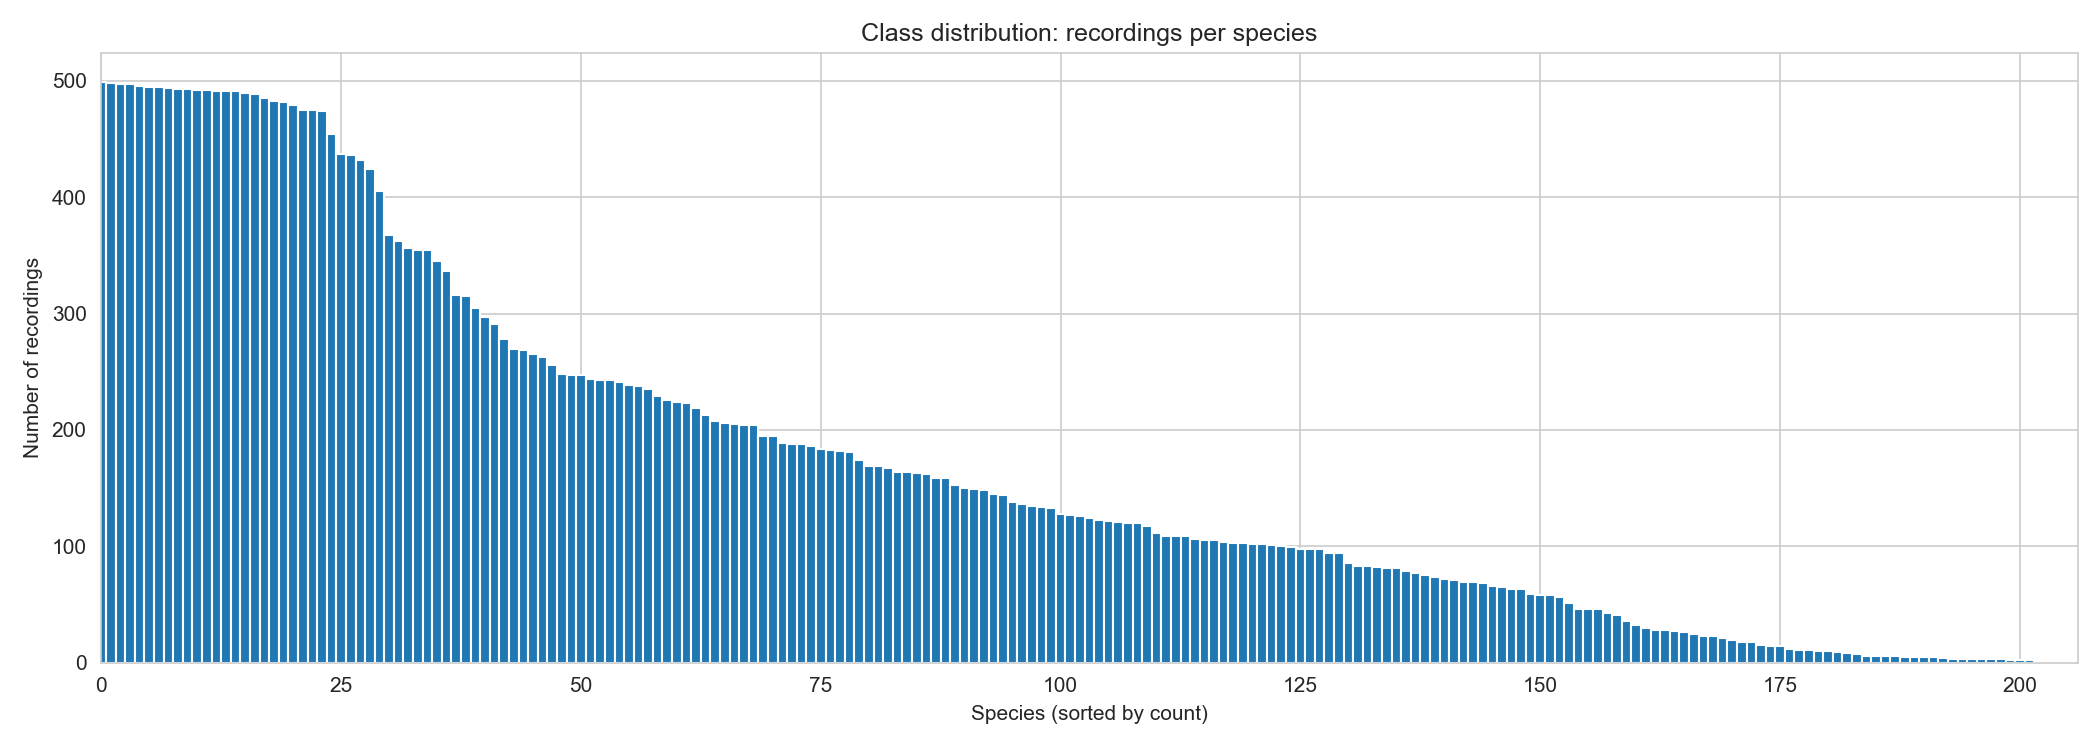
\includegraphics[width=0.85\textwidth]{../figures/class_distribution.png}
    \caption{Number of recordings per species, sorted in descending order. The long tail shows that many species have very few training examples.}
    \label{fig:class_dist}
\end{figure}

\subsection{Taxonomic breakdown}

The dataset is dominated by birds (162 species, 34,799 recordings). Amphibians, insects, mammals, and reptiles make up the remaining 72 species but only 750 recordings combined. This imbalance means the model will be much more exposed to bird vocalizations during training.

\begin{figure}[H]
    \centering
    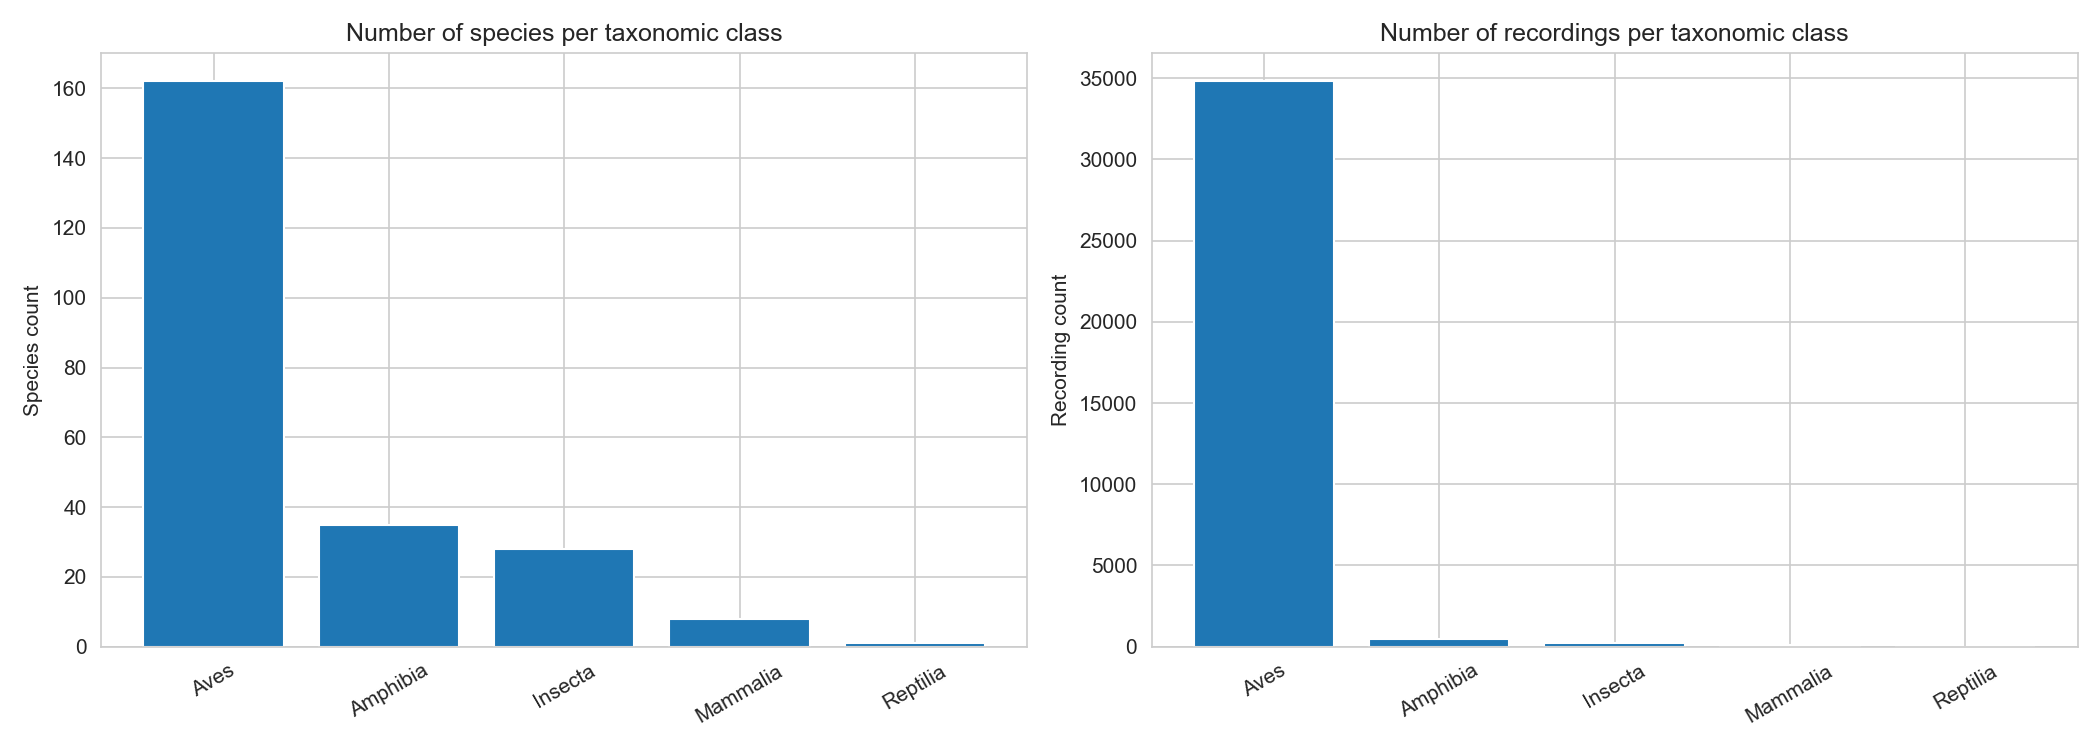
\includegraphics[width=0.85\textwidth]{../figures/taxonomic_distribution.png}
    \caption{Number of species and recordings per taxonomic class. Birds dominate both in diversity and data volume.}
    \label{fig:tax_dist}
\end{figure}

\subsection{Soundscape characteristics}

The labeled soundscape segments are multi-label, with an average of about 4--5 species per 5-second window (Figure~\ref{fig:sps}). This reflects the reality of field recordings where many animals call simultaneously. I noticed 28 species that appear in the soundscape labels but not in train\_audio — these are species I cannot train on directly.

\begin{figure}[H]
    \centering
    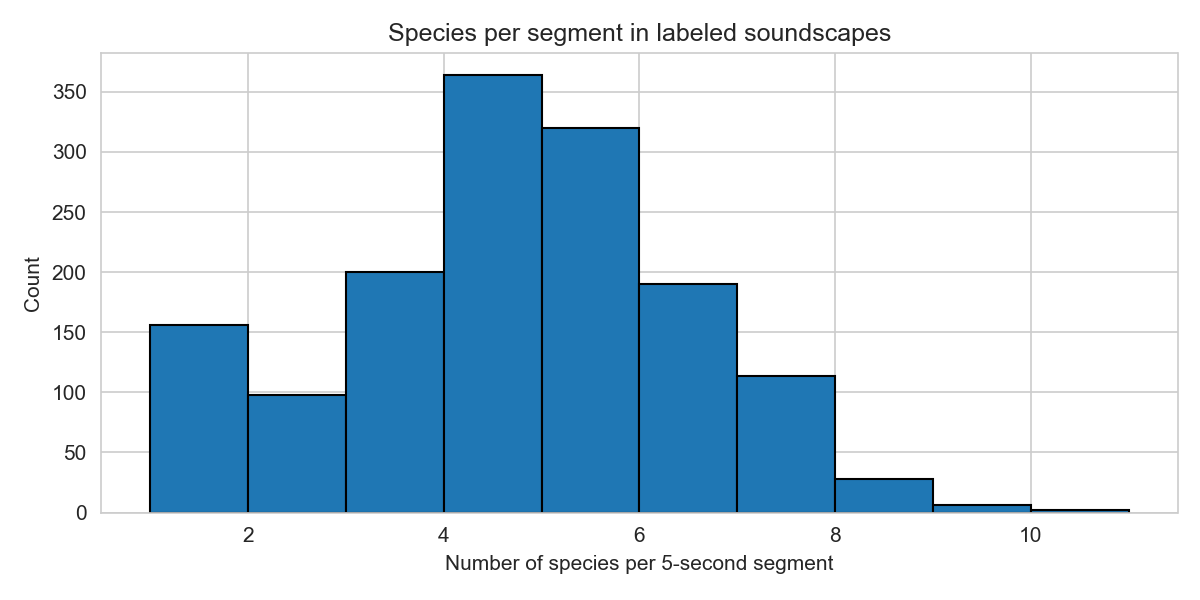
\includegraphics[width=0.6\textwidth]{../figures/species_per_segment.png}
    \caption{Distribution of the number of species per 5-second soundscape segment.}
    \label{fig:sps}
\end{figure}

\subsection{Domain gap}

Looking at spectrograms of clean training clips vs.\ soundscape segments, the difference is obvious. Training clips are typically close-up recordings of a single species with little background noise. Soundscapes contain overlapping calls, wind, insects buzzing, and generally much more noise. This domain shift is one of the main challenges.

\begin{figure}[H]
    \centering
    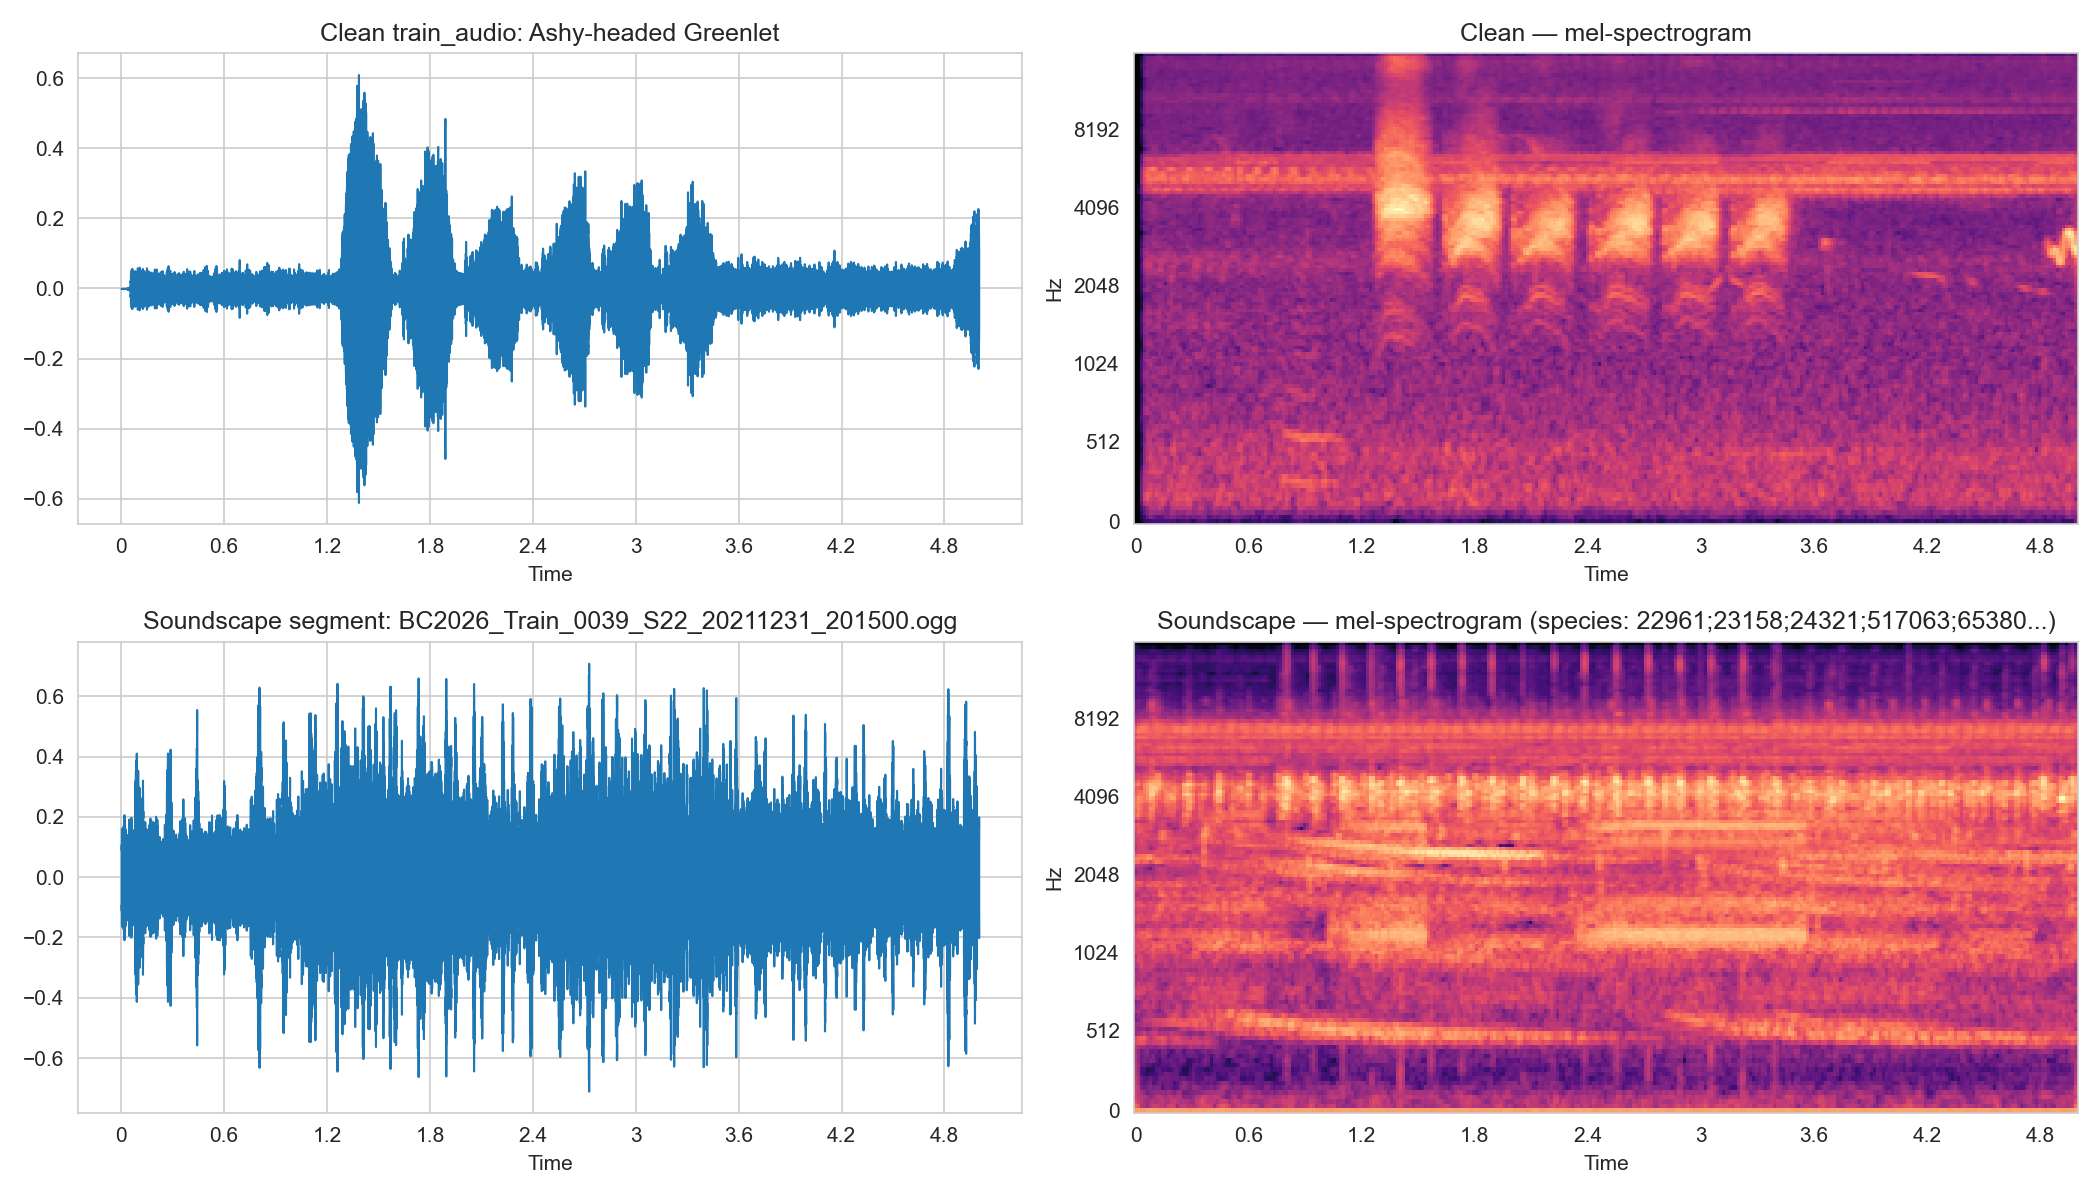
\includegraphics[width=0.85\textwidth]{../figures/clean_vs_noisy.png}
    \caption{Comparison of a clean training clip (top) and a soundscape segment (bottom). The soundscape is noisier with multiple overlapping signals.}
    \label{fig:domain_gap}
\end{figure}

% ============================================================
\section{Methodology}

\subsection{Feature engineering}

Since I cannot use neural networks to learn features automatically, I used the \texttt{librosa} library to extract hand-crafted audio features. For each recording, I computed the following features across all time frames:

\begin{itemize}
    \item \textbf{MFCCs} (13 coefficients): capture the spectral envelope — the overall shape of the frequency content. This is the most important feature for audio classification because different species produce different frequency patterns.
    \item \textbf{Spectral centroid}: the ``center of mass'' of the spectrum — indicates whether the sound is high-pitched or low-pitched.
    \item \textbf{Spectral bandwidth}: how spread out the frequencies are. A pure tone has narrow bandwidth; noise has wide bandwidth.
    \item \textbf{Spectral rolloff}: the frequency below which most of the energy lies.
    \item \textbf{Zero-crossing rate (ZCR)}: how often the signal changes sign. Buzzing insects have high ZCR; low tones have low ZCR.
    \item \textbf{RMS energy}: the overall loudness of the signal.
    \item \textbf{Chroma features} (12 bins): distribution of energy across the 12 pitch classes (C, C\#, ..., B).
\end{itemize}

Since audio clips have different lengths, I aggregated each feature over time using summary statistics. I tested two approaches:

\begin{itemize}
    \item \textbf{SET\_C} (60 features): mean and standard deviation for each of the 30 raw features.
    \item \textbf{SET\_D} (180 features): mean, standard deviation, minimum, maximum, 25th percentile, and 75th percentile. This captures more about how features vary over time.
\end{itemize}

\subsection{Models}

I picked five classical models that together cover the main families of classifiers, so the comparison would actually be informative. For each one I describe both what it is and why it makes sense to try on this problem.

\begin{itemize}
    \item \textbf{Random Forest} (100 trees): ensemble of decision trees built with bagging. Chosen as the main baseline because it handles high-dimensional features well, does not require scaling, naturally handles multi-class problems, and provides feature importance scores — which are useful for the ablation study.
    \item \textbf{Logistic Regression} (L2-regularized): a simple linear model. Included to test whether the engineered feature space is approximately linearly separable. If a linear model performs well, it means most of the discriminative work was already done by the feature extraction step. Features were standardized using StandardScaler since scale matters for regularization.
    \item \textbf{Linear SVM}: another linear baseline, but with a different loss function (hinge loss instead of log loss). I used a linear kernel rather than RBF because RBF kernels scale roughly as $O(n^2)$ with the number of samples, which is impractical for 35,000 training points. Comparing two linear models with different losses tells me whether the choice of loss matters here.
    \item \textbf{LightGBM}: gradient boosting decision trees, generally considered the state of the art for tabular data. Included to test whether more complex non-linear feature interactions help beyond what Random Forest captures with bagging.
    \item \textbf{k-NN} ($k=5$): non-parametric baseline, classifies based on distance to nearest training points. I expect it to perform poorly here because of the curse of dimensionality at 180 features, but including it gives a useful weak baseline for comparison.
\end{itemize}

Together these models cover: tree ensembles (RF, LightGBM), linear models (LogReg, SVM), and distance-based methods (k-NN). The comparison should reveal which family is best suited to this kind of feature space.

\subsection{Evaluation}

I used three metrics:
\begin{itemize}
    \item \textbf{Accuracy}: fraction of correct top-1 predictions.
    \item \textbf{Macro F1}: F1 score averaged equally across all classes. Sensitive to class imbalance.
    \item \textbf{Macro ROC-AUC}: area under the ROC curve, computed in a one-vs-rest manner and averaged across all classes that have both positive and negative examples in the validation fold. This is the primary metric — it measures ranking quality rather than hard decisions.
\end{itemize}

For model comparison, I used 5-fold stratified cross-validation to get reliable estimates. Species with fewer than 2 samples were excluded since stratified splitting requires at least 2 per class.

For soundscape evaluation, since my model predicts a single species but soundscapes are multi-label, I used a simplified ``top-1 hit rate'': I checked whether the model's prediction is among the true species listed for that segment. This underestimates performance but gives a rough measure of generalization.

% ============================================================
\section{Experiments and Results}

\subsection{Baseline}

I started with a Random Forest (100 trees, default parameters) on SET\_C features (60 features). This gave:

\begin{table}[H]
\centering
\begin{tabular}{lc}
\toprule
Metric & Value \\
\midrule
Accuracy & 21.6\% \\
Macro F1 & 0.176 \\
Macro ROC-AUC & 0.744 \\
Soundscape hit rate & 2.3\% \\
Training time & 8s \\
\bottomrule
\end{tabular}
\caption{Baseline results (Random Forest, SET\_C features).}
\label{tab:baseline}
\end{table}

The accuracy looks low, but with 202 classes random guessing would give about 0.5\%, so the model is roughly 40 times better than chance. The ROC-AUC of 0.744 confirms that the features carry meaningful information.

The feature importance plot (Figure~\ref{fig:feat_imp}) shows which features the Random Forest relies on most:

\begin{figure}[H]
    \centering
    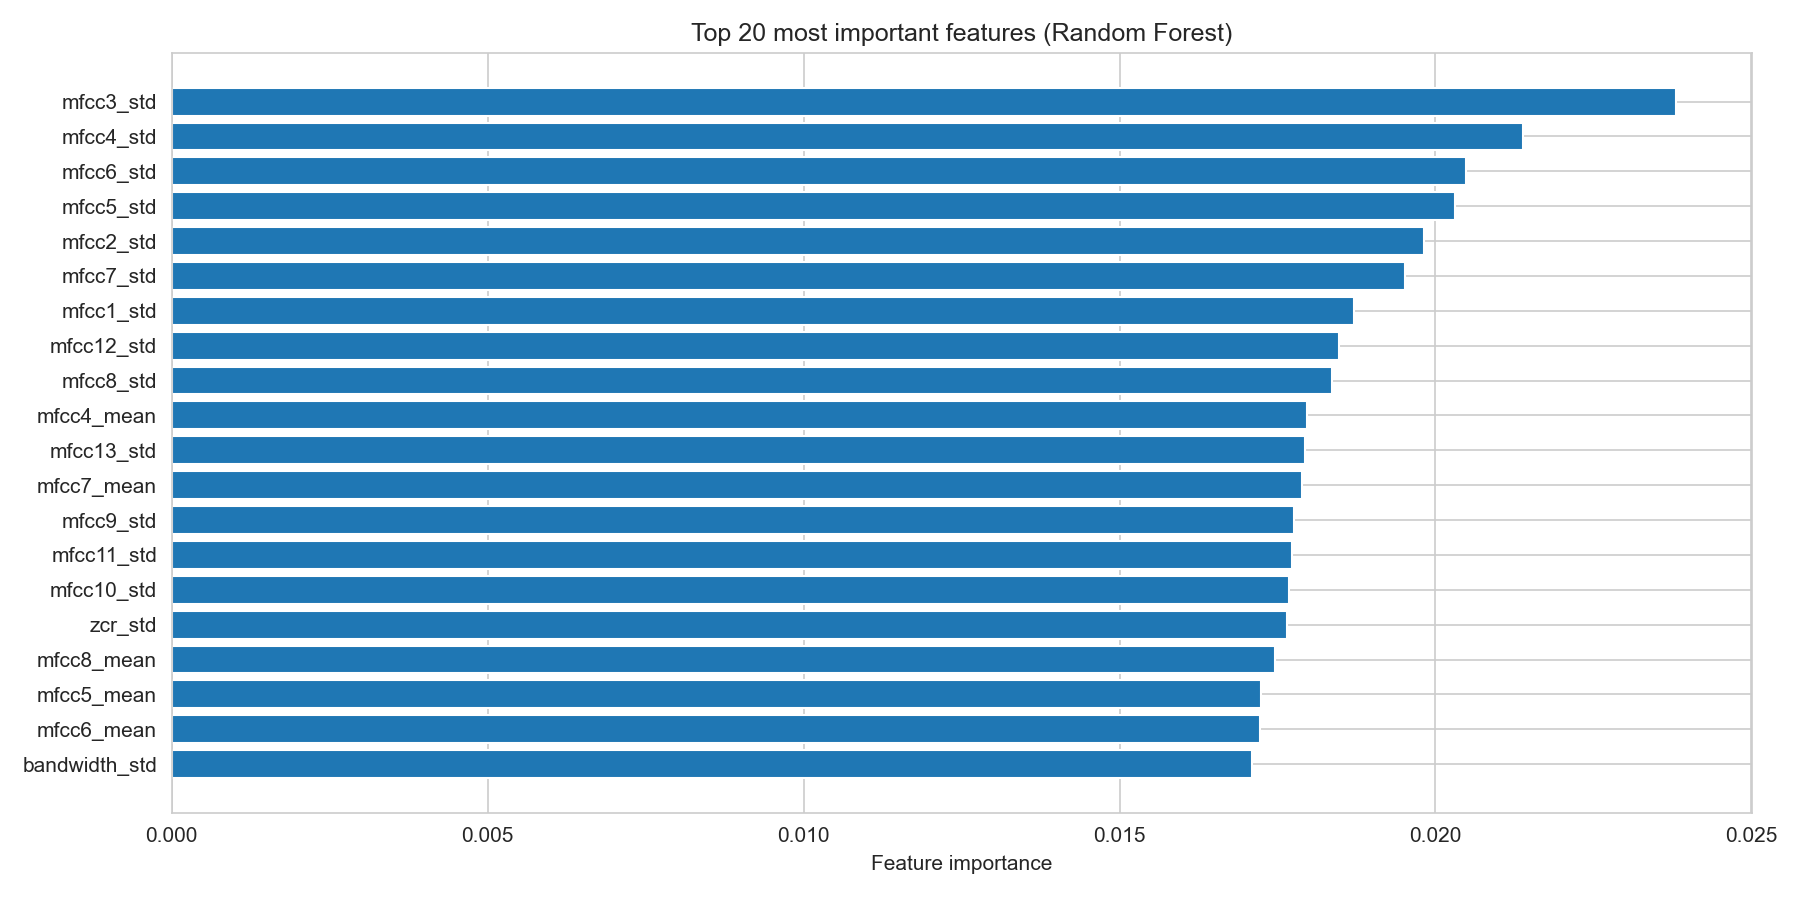
\includegraphics[width=0.75\textwidth]{../figures/feature_importance_baseline.png}
    \caption{Top 20 most important features in the baseline Random Forest. MFCC features dominate.}
    \label{fig:feat_imp}
\end{figure}

\subsection{Feature comparison}

I compared four feature sets, all using the same Random Forest model:

\begin{table}[H]
\centering
\begin{tabular}{lccccc}
\toprule
Feature set & Features & Accuracy & Macro F1 & ROC-AUC & Time \\
\midrule
SET\_A (MFCCs only) & 26 & 20.8\% & 0.161 & 0.747 & 5.7s \\
SET\_B (+spectral) & 36 & 20.9\% & 0.169 & 0.755 & 6.4s \\
SET\_C (+chroma) & 60 & 21.6\% & 0.176 & 0.744 & 7.6s \\
SET\_D (extended) & 180 & 25.0\% & 0.203 & 0.772 & 13.9s \\
\bottomrule
\end{tabular}
\caption{Feature set comparison. All experiments use the same Random Forest model.}
\label{tab:features}
\end{table}

MFCCs alone already give a ROC-AUC of 0.747, confirming they are the most informative features. Adding spectral features helps slightly. Chroma features actually decreased ROC-AUC, suggesting pitch-class information is not very useful for animal vocalizations. The biggest improvement came from SET\_D's extended statistics — capturing min, max, and percentiles helps the model understand how features change over time, not just their average.

\begin{figure}[H]
    \centering
    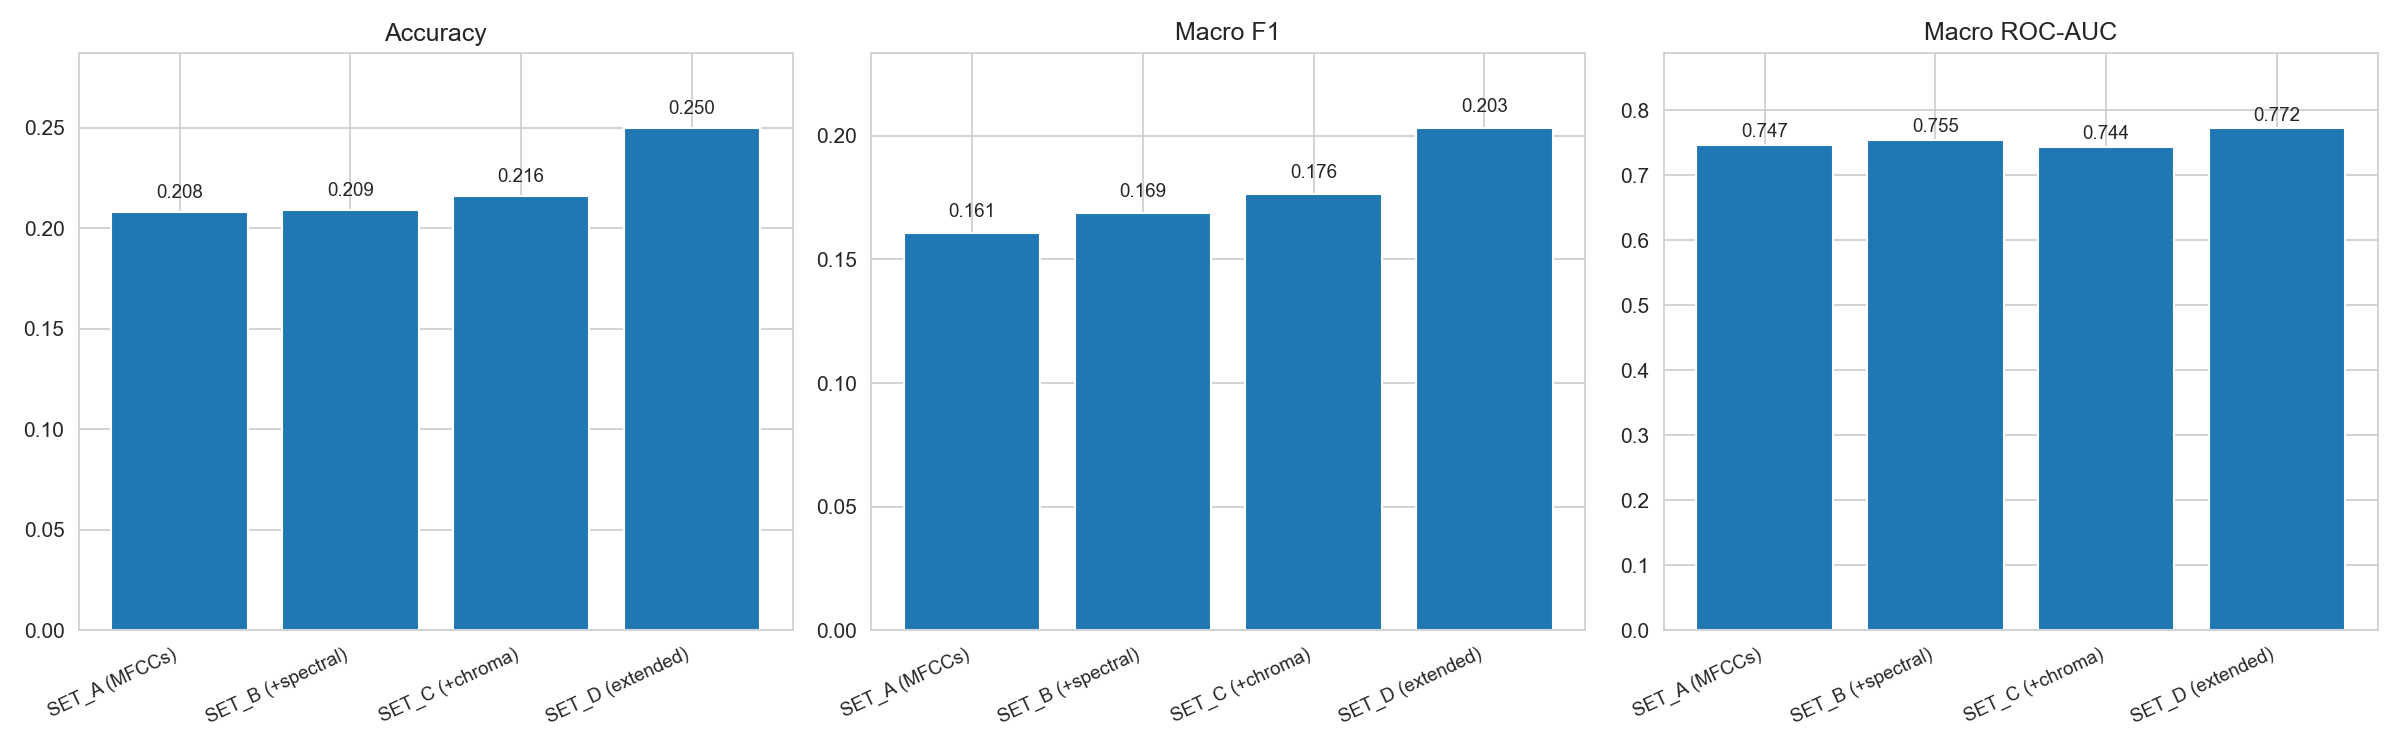
\includegraphics[width=0.85\textwidth]{../figures/feature_comparison.png}
    \caption{Comparison of feature sets across all three metrics.}
    \label{fig:feat_comp}
\end{figure}

\subsection{Model comparison}

Using SET\_D features, I compared five models with 5-fold stratified cross-validation:

\begin{table}[H]
\centering
\begin{tabular}{lcccc}
\toprule
Model & Accuracy & Macro F1 & ROC-AUC & Time \\
\midrule
Random Forest & 0.256 $\pm$ 0.005 & 0.200 $\pm$ 0.010 & 0.770 $\pm$ 0.005 & 69s \\
Logistic Regression & \textbf{0.328 $\pm$ 0.003} & \textbf{0.270 $\pm$ 0.007} & \textbf{0.893 $\pm$ 0.004} & 76s \\
Linear SVM & 0.306 $\pm$ 0.004 & 0.230 $\pm$ 0.005 & 0.867 $\pm$ 0.003 & 666s \\
LightGBM (default) & 0.018 $\pm$ 0.004 & 0.008 $\pm$ 0.007 & 0.504 $\pm$ 0.003 & 96s \\
k-NN ($k$=5) & 0.151 $\pm$ 0.005 & 0.129 $\pm$ 0.009 & 0.639 $\pm$ 0.005 & $<$1s \\
\bottomrule
\end{tabular}
\caption{Model comparison with 5-fold stratified CV on SET\_D features. Mean $\pm$ std shown.}
\label{tab:models}
\end{table}

The most surprising result is that Logistic Regression clearly outperformed everything else, including Random Forest. This goes directly against hypothesis H2 (non-linear models should win because of class complexity), so it is worth analysing carefully.

A bias-variance interpretation helps here. The 180 features are summary statistics computed over time (mean, std, min, max, percentiles of MFCCs and other descriptors). The non-linear transformation from raw audio to features is therefore done \textit{before} the classifier sees the data. By the time the classifier receives the input, most of the work is already done — the remaining task is mostly to draw separating boundaries in a fixed representation. In this regime, the bottleneck is not the model's ability to capture complex patterns (bias) but rather its ability to generalize from finite samples per species (variance). A linear model has lower variance than Random Forest or LightGBM, and that pays off here.

The Random Forest vs LightGBM comparison is also informative. Both are tree ensembles, but they reduce error in different ways: Random Forest uses bagging (independent trees on bootstrap samples, then averaging), while LightGBM uses boosting (sequential trees, each fitting the residual errors of the previous ones). Bagging mainly reduces variance, while boosting can reduce both bias and variance but is much more sensitive to hyperparameters. This explains why LightGBM with default settings failed catastrophically (ROC-AUC $\approx$ 0.50), while Random Forest worked reasonably out of the box. With 202 classes and default settings, LightGBM's learning rate is simply too high — each tree overshoots the optimum. Lowering it and adding more trees recovered most of the performance (see Section~4.4), but the model never quite matched Logistic Regression.

k-NN performed poorly because of the curse of dimensionality — with 180 features, distances between points become uniform and the notion of ``nearest neighbour'' loses meaning. This is a well-known issue and the result is consistent with what the lectures predicted for high-dimensional spaces.

\begin{figure}[H]
    \centering
    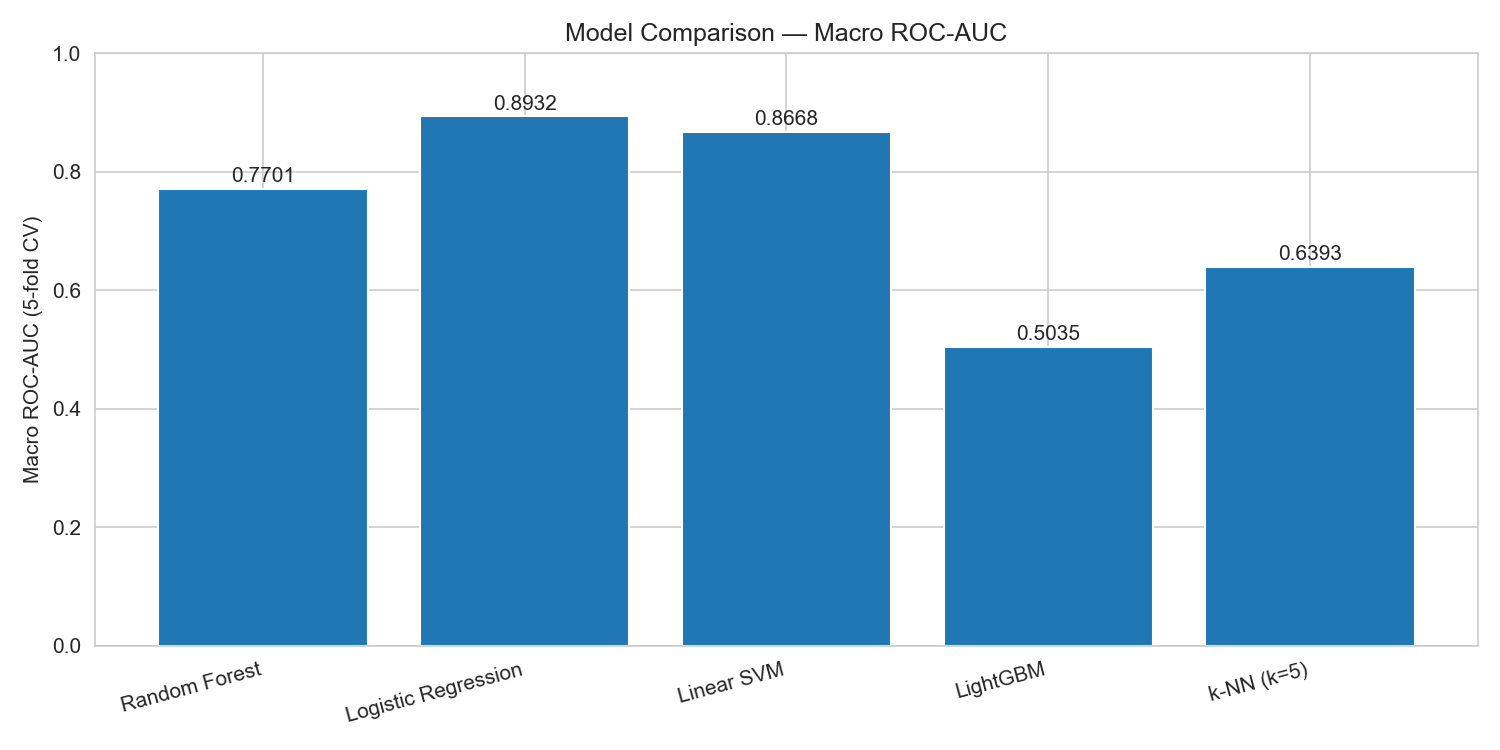
\includegraphics[width=0.7\textwidth]{../figures/model_comparison.png}
    \caption{ROC-AUC comparison across models.}
    \label{fig:model_comp}
\end{figure}

\subsection{Hyperparameter tuning}

I tuned Logistic Regression's regularization parameter $C$ by testing values from 0.001 to 10:

\begin{figure}[H]
    \centering
    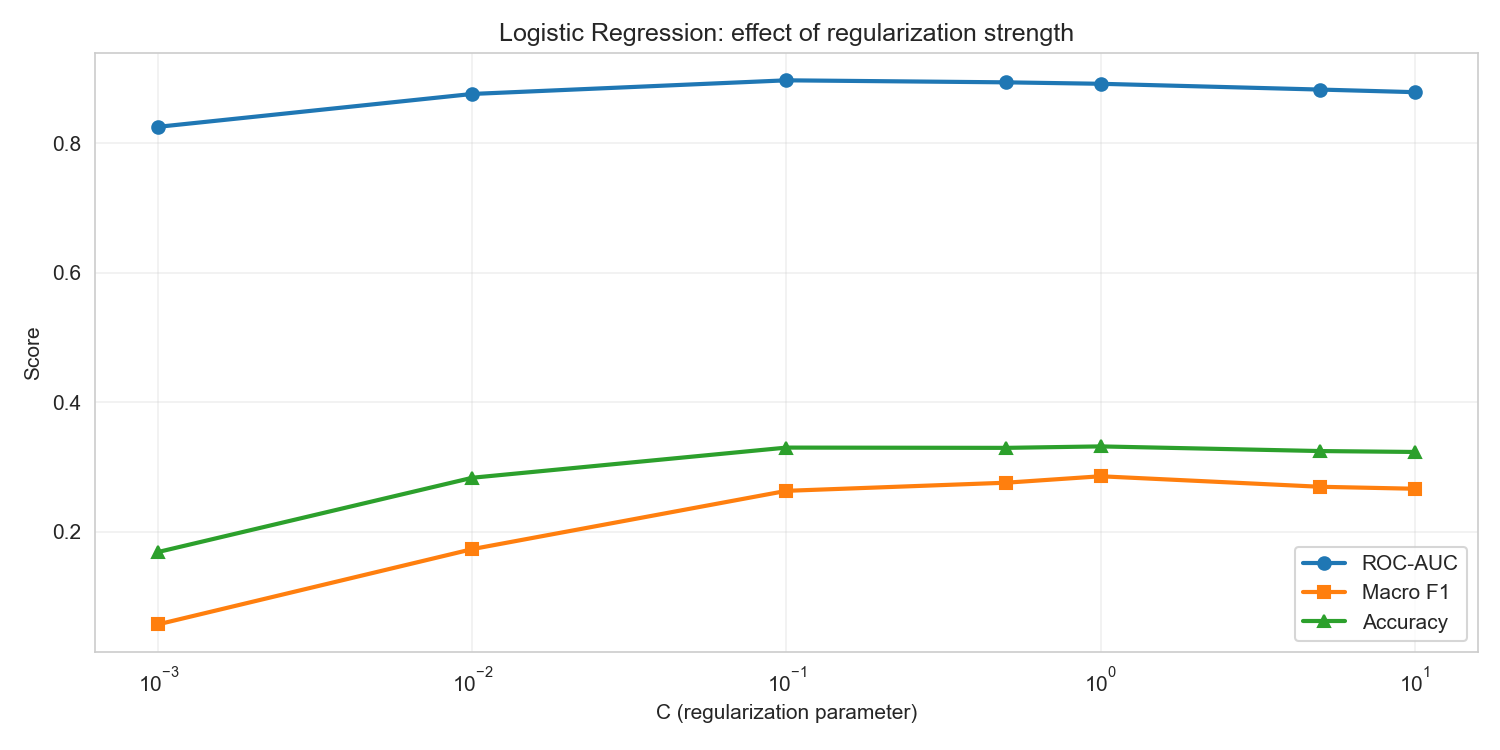
\includegraphics[width=0.7\textwidth]{../figures/lr_tuning.png}
    \caption{Effect of regularization strength on Logistic Regression. Best ROC-AUC at $C = 0.1$.}
    \label{fig:lr_tuning}
\end{figure}

The best value was $C = 0.1$ with ROC-AUC = 0.897, a small improvement over the default $C = 1.0$ (0.892). The model is not very sensitive to this parameter in the 0.1--1.0 range, but very low $C$ hurts because the model is over-regularized.

I also tried to fix LightGBM by increasing the number of trees and lowering the learning rate. The key finding was that both changes were needed together:

\begin{table}[H]
\centering
\begin{tabular}{lccc}
\toprule
Configuration & Accuracy & ROC-AUC & Time \\
\midrule
100 trees, lr=0.1 (default) & 1.5\% & 0.501 & 19s \\
300 trees, lr=0.1 & 1.5\% & 0.501 & 42s \\
300 trees, lr=0.05 & 3.6\% & 0.517 & 53s \\
500 trees, lr=0.05 & 3.6\% & 0.517 & 80s \\
500 trees, lr=0.01 & 30.1\% & 0.865 & 419s \\
\bottomrule
\end{tabular}
\caption{LightGBM with different configurations. Only the combination of many trees \textit{and} a low learning rate produced good results.}
\label{tab:lgbm}
\end{table}

With 500 trees and learning rate 0.01, LightGBM recovered to a ROC-AUC of 0.865 — competitive but still below Logistic Regression (0.897), and much slower (419s vs 76s).

\subsection{Adding non-audio metadata}

The \texttt{train.csv} file contains useful non-audio information about each recording: latitude, longitude, a quality rating (0--5), and a categorical \texttt{collection} field indicating whether the recording came from Xeno-canto (XC) or iNaturalist (iNat). I wanted to check whether adding this metadata to the audio features helps, since species have known geographic ranges and recording quality should correlate with how clean the audio is.

I built a small metadata block of four features (lat, lon, rating, and a binary \texttt{is\_inat} flag) and concatenated it with the 180-d audio feature vector to get a 184-d combined input. I re-ran Logistic Regression with the same 5-fold stratified CV protocol for a clean comparison.

\begin{table}[H]
\centering
\begin{tabular}{lccc}
\toprule
Feature set & Accuracy & Macro F1 & ROC-AUC \\
\midrule
Audio only (180 features) & 0.328 $\pm$ 0.003 & 0.270 $\pm$ 0.007 & 0.893 $\pm$ 0.004 \\
Audio + metadata (184 features) & \textbf{0.377 $\pm$ 0.004} & \textbf{0.315 $\pm$ 0.010} & \textbf{0.922 $\pm$ 0.004} \\
\bottomrule
\end{tabular}
\caption{Effect of adding four non-audio metadata features (latitude, longitude, rating, collection source) to the audio feature set. Logistic Regression, 5-fold stratified CV.}
\label{tab:metadata}
\end{table}

\begin{figure}[H]
    \centering
    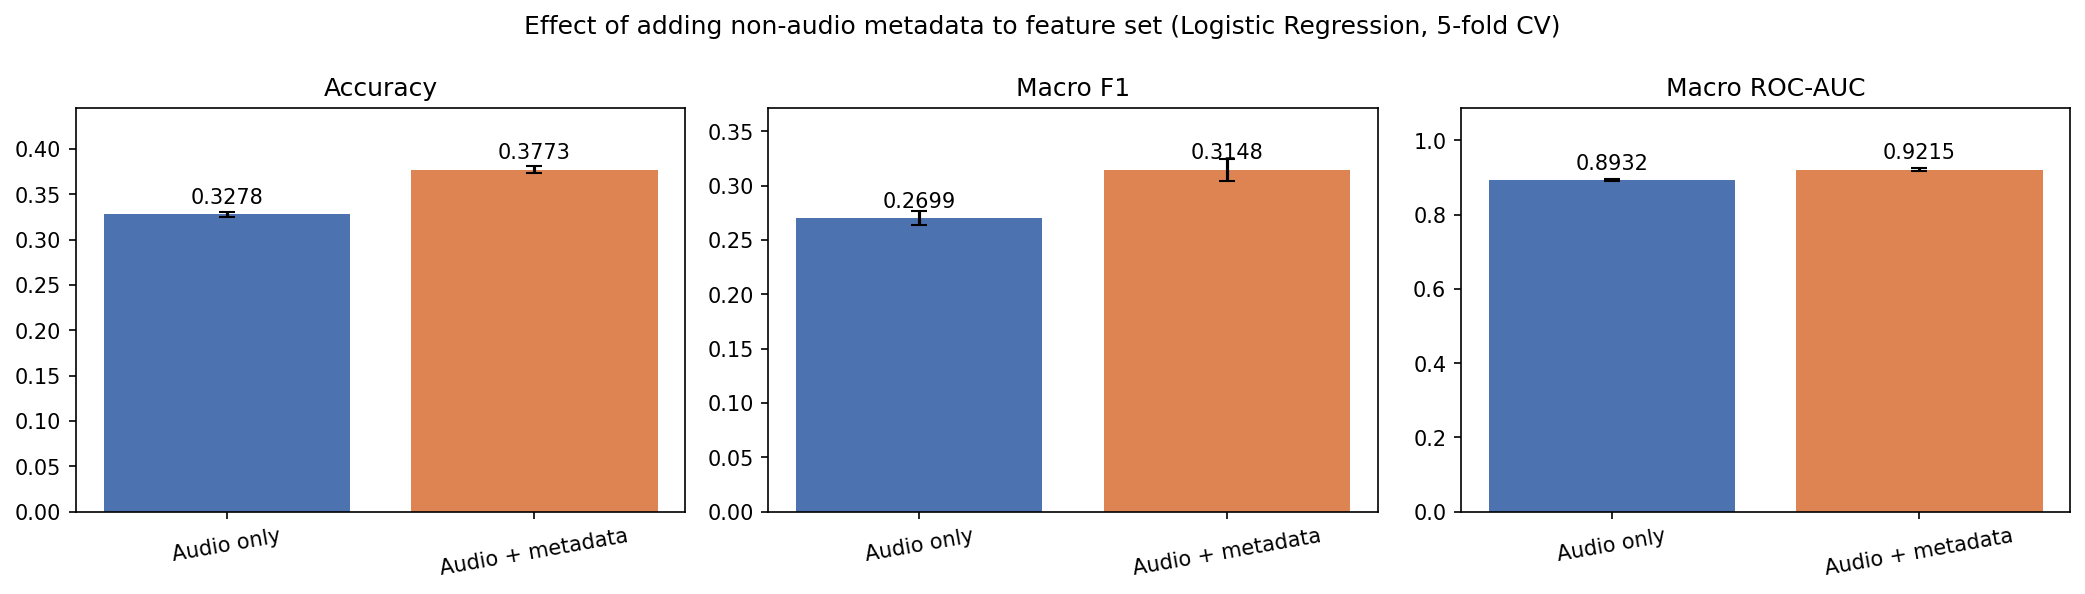
\includegraphics[width=0.95\textwidth]{../figures/metadata_comparison.png}
    \caption{Comparison of Logistic Regression with and without non-audio metadata features.}
    \label{fig:metadata}
\end{figure}

The improvement was larger than I expected. ROC-AUC went from 0.893 to 0.922 ($+$0.029), and top-1 accuracy jumped from 32.8\% to 37.7\% ($+$4.9 percentage points). For just four extra features, this is a substantial gain. Two reasons probably explain it:

\begin{itemize}
    \item \textbf{Geographic prior}: latitude and longitude essentially encode a species range prior. Some species are common in one part of the Pantanal and absent in others. A linear classifier can use the lat/lon coefficients to push up the probability of locally-common species and down for ones that are not expected at that location.
    \item \textbf{Quality signal}: the rating field correlates with how clean the recording is. A high-rated recording's audio features are more reliable, so the classifier can effectively learn to trust them more.
\end{itemize}

It is worth pointing out that this works under realistic deployment conditions: in the field, the recorders have fixed known locations, so lat/lon would be available at inference time too. The rating field would not be available for unlabeled test data, but lat/lon alone likely carries most of the benefit.

\subsection{Ablation study}

To understand which feature groups matter most, I removed one group at a time and measured the drop in ROC-AUC:

\begin{figure}[H]
    \centering
    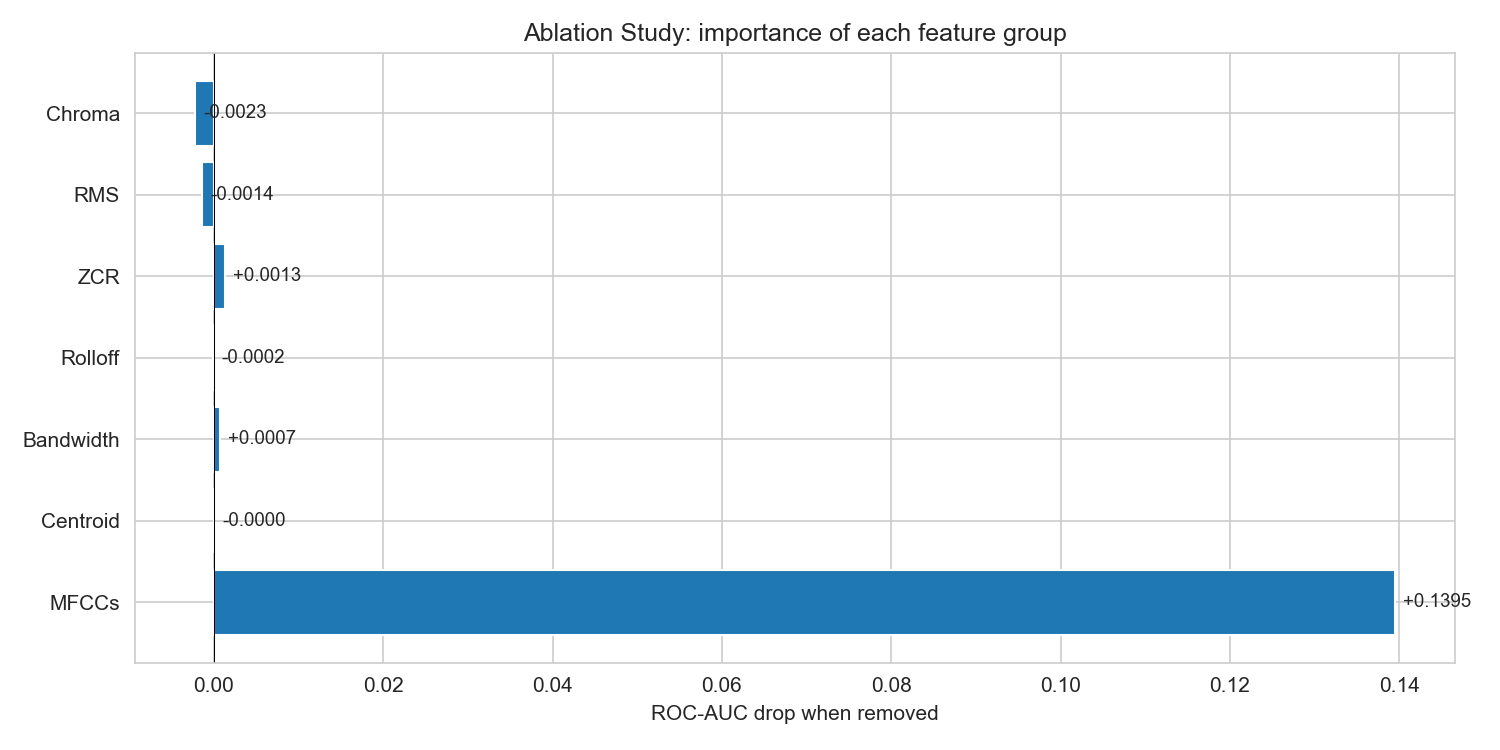
\includegraphics[width=0.7\textwidth]{../figures/ablation_study.png}
    \caption{ROC-AUC drop when each feature group is removed. MFCCs are by far the most important.}
    \label{fig:ablation}
\end{figure}

Removing MFCCs drops ROC-AUC by 0.14 (from 0.897 to 0.758). All other feature groups individually contribute less than 0.002 — centroid, bandwidth, rolloff, ZCR, RMS, and chroma have almost no effect when removed. This confirms that MFCCs carry the vast majority of useful information for species classification.

Interestingly, removing chroma actually slightly improves ROC-AUC, consistent with the feature comparison where adding chroma to SET\_B didn't help.

\subsection{Error analysis}

I looked at which species are hardest to classify. Species with fewer training samples generally have lower per-class ROC-AUC, confirming that class imbalance hurts performance.

\begin{figure}[H]
    \centering
    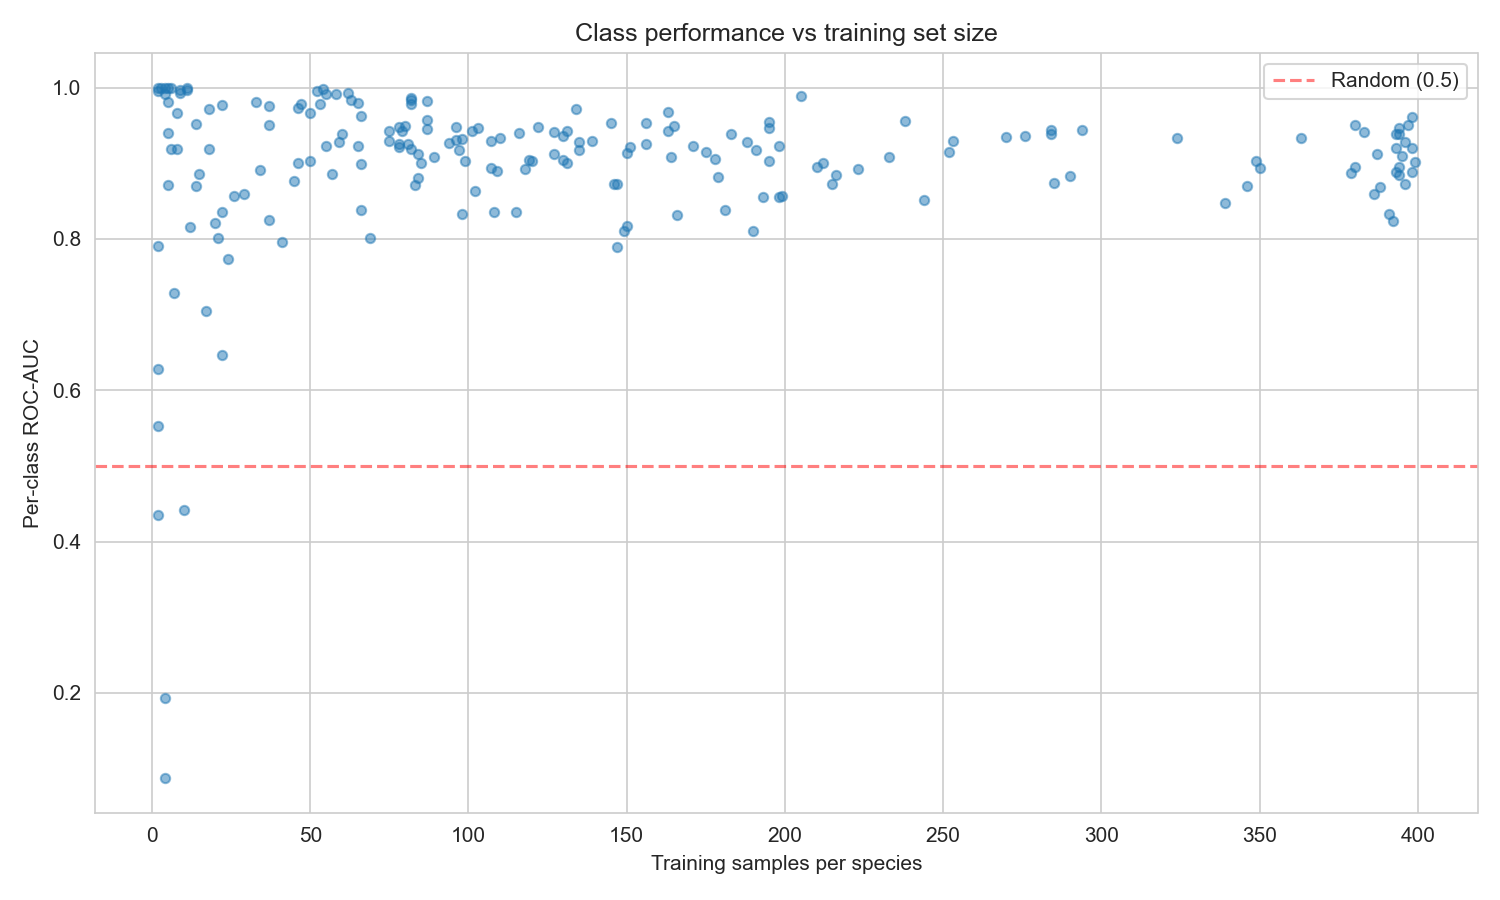
\includegraphics[width=0.7\textwidth]{../figures/class_size_vs_auc.png}
    \caption{Per-class ROC-AUC vs.\ number of training samples. Species with very few samples tend to perform worse.}
    \label{fig:class_size}
\end{figure}

The confusion matrix for the 15 most common species (Figure~\ref{fig:confusion}) shows that confusion tends to happen between acoustically similar species. This suggests that hand-crafted features struggle to capture subtle differences between species that produce similar frequency patterns — a limitation that deep learning approaches could potentially overcome.

\begin{figure}[H]
    \centering
    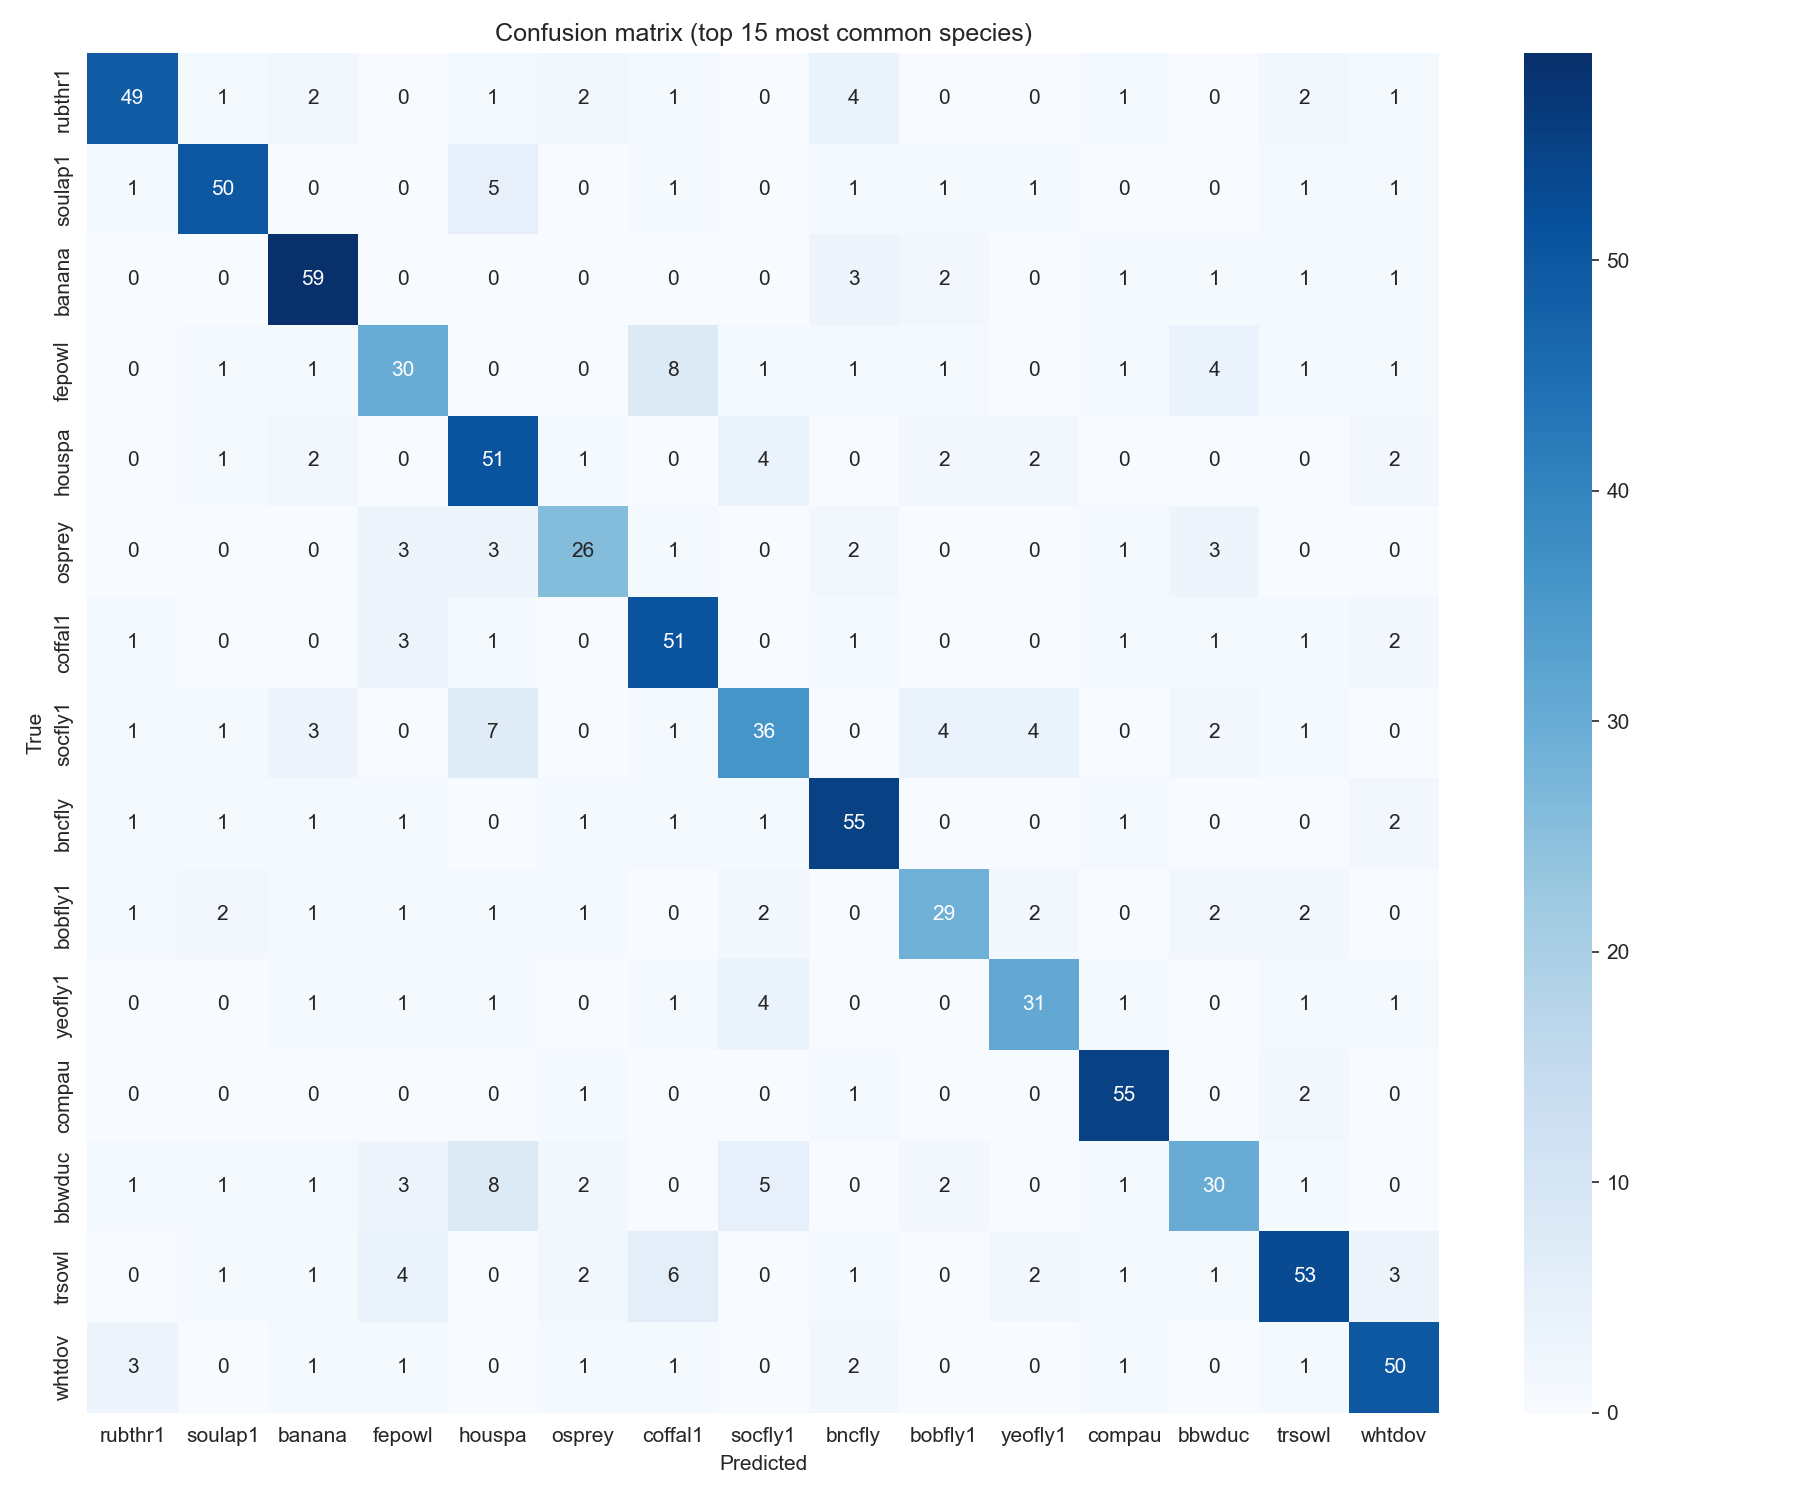
\includegraphics[width=0.8\textwidth]{../figures/confusion_matrix_top15.png}
    \caption{Confusion matrix for the 15 most common species. Off-diagonal values indicate confusion between species pairs.}
    \label{fig:confusion}
\end{figure}

\subsection{Taxonomic performance}

Performance varies across taxonomic groups, as expected since different animal classes produce very different types of sounds.

\begin{figure}[H]
    \centering
    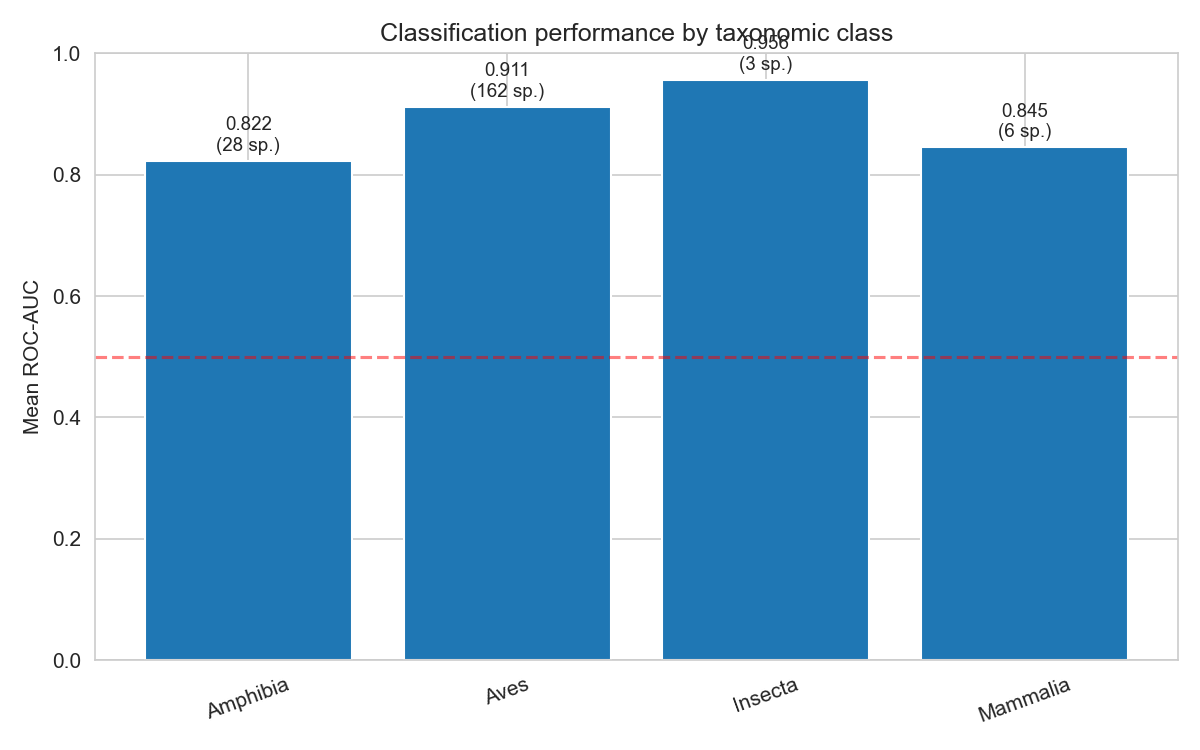
\includegraphics[width=0.65\textwidth]{../figures/performance_by_taxon.png}
    \caption{Mean ROC-AUC by taxonomic class.}
    \label{fig:taxon}
\end{figure}

\subsection{Domain shift}

I compared model performance on clean validation data (train\_audio) vs.\ noisy field recordings (labeled soundscapes). For a fair comparison, I used SET\_C features for both (since SET\_D was not extracted for soundscapes) and retrained Logistic Regression accordingly.

\begin{itemize}
    \item Validation accuracy: 25.5\%, ROC-AUC: 0.870
    \item Soundscape top-1 hit rate: 8.8\%
\end{itemize}

The roughly 3x drop in performance reflects the differences in noise, overlapping species, and recording conditions between curated training audio and real-world soundscapes. Still, the soundscape hit rate improved from 2.3\% (initial RF baseline) to 8.8\% with a better model, showing that improvements on clean data do transfer partially.

% ============================================================
\section{Discussion}
\label{sec:discussion}

\subsection{Revisiting the hypotheses}

The three hypotheses from Section~1 are answered by the experiments:

\begin{itemize}
    \item \textbf{H1 (MFCCs dominate): confirmed.} The ablation study showed that removing MFCCs alone drops ROC-AUC by 0.14, while removing any other feature group changes it by less than 0.002. MFCCs are designed specifically to compress the spectral envelope into a small set of perceptually meaningful coefficients, so this result is expected — but the magnitude of dominance was larger than I anticipated.
    \item \textbf{H2 (non-linear models win): falsified.} Logistic Regression beat both Random Forest and LightGBM. This was the most interesting finding and is discussed below.
    \item \textbf{H3 (significant domain shift): confirmed.} Top-1 accuracy dropped from 25.5\% on clean validation data to 8.8\% on noisy soundscapes — roughly a 3x drop in performance, consistent with the visual differences between the two distributions.
\end{itemize}

\subsection{Key findings}

The most interesting finding is that Logistic Regression outperformed all other models, including ensemble methods. The intuition is that feature engineering already did the non-linear work that ensemble methods would normally learn — once you summarize an audio clip into 180 statistics, what is left is mostly linear separation between species. In that setting, simpler models with lower variance generalize better than complex ones, which matches what was discussed in the bias-variance lectures.

Another important finding is how much MFCCs dominate. The ablation study showed that all other feature groups combined contribute less than 2\% of the total information. This makes sense — MFCCs are specifically designed to represent the spectral envelope in a compact, perceptually meaningful way. It also suggests that chroma and other features could be dropped without much loss, which would speed up the pipeline considerably.

A third finding worth mentioning is that hyperparameter sensitivity varied a lot between models. Logistic Regression was barely affected by the choice of $C$ (within the 0.1--1.0 range), while LightGBM required substantial tuning just to escape the random-prediction regime. This is consistent with what was covered in lecture on ensemble methods: boosting is more sensitive to hyperparameters than bagging.

\subsection{Limitations}

There are several limitations to this work:

\begin{itemize}
    \item \textbf{Single-label simplification}: the real problem is multi-label (multiple species per segment), but I treated it as single-label. A proper multi-label approach using OneVsRestClassifier with 234 binary classifiers would be more appropriate, but the limited labeled soundscape data (1,478 segments for 234 species) makes this challenging.
    \item \textbf{Domain shift}: the biggest bottleneck is the gap between clean training audio and noisy field recordings. My features don't account for background noise or overlapping signals.
    \item \textbf{Missing species}: 28 target species have no training audio. A model cannot learn to recognize what it has never seen.
    \item \textbf{No temporal dynamics}: my features aggregate each clip into static summary statistics (mean, std, min/max, percentiles). This throws away the temporal structure of a call — its rhythm, attack, and decay. Features like delta-MFCCs or RNN-style sequence modelling could capture this, but neither was feasible here.
    \item \textbf{No statistical significance testing}: the model comparison reports mean $\pm$ std across CV folds, but I did not formally test whether the differences between models are statistically significant. Bootstrap confidence intervals or a paired test would make the comparison more defensible.
    \item \textbf{Chroma features may be ill-suited}: chroma was originally designed for music analysis (where pitch class matters). For broadband animal sounds like insect buzzes, it likely adds noise rather than signal — which is consistent with the ablation result showing that removing chroma slightly \textit{improved} ROC-AUC.
    \item \textbf{No neural networks}: modern approaches using CNNs on spectrograms or pretrained audio models typically achieve much higher performance on these tasks. The hand-crafted features, while effective, cannot capture the complex temporal and spectral patterns that deep learning can learn automatically.
\end{itemize}

\subsection{On the use of pre-trained models}

Although the project's no-neural-networks constraint ruled out training any deep model from scratch, it is worth discussing where pre-trained models would fit into a pipeline like this one. The most relevant model for this task is BirdNET (Cornell Lab of Ornithology), a CNN trained on millions of labeled bird recordings, which is widely considered the state-of-the-art for bird acoustic identification. There are two distinct ways it could be used:

\begin{enumerate}
    \item \textbf{As a direct baseline:} run BirdNET inference on the same audio and compare its species predictions to mine. This would give an upper bound on what is achievable on this task with deep learning, and would put my 0.897 ROC-AUC in context. The catch is that BirdNET only covers around 3,000 bird species — it has no coverage for the amphibians, mammals, reptiles, or insect sonotypes that make up part of the BirdCLEF+ 2026 target set. A direct comparison would only be possible on the bird subset.
    \item \textbf{As a feature extractor:} extract BirdNET's intermediate embeddings (e.g.\ from its penultimate layer) and use them as input to a classical classifier like the Logistic Regression I trained. This would combine the representational power of deep learning with the simplicity and interpretability of a linear classifier. Because no NN training is involved — only inference — this approach would arguably still respect the spirit of the constraint, while likely producing substantially better results.
\end{enumerate}

I did not run either experiment, partly because of time and partly because the no-neural-networks rule was unclear about pure inference. But the methodological point is that classical ML and pre-trained deep learning are not mutually exclusive: there is a hybrid pipeline that uses pre-trained embeddings as features and a classical classifier on top, which would be a natural next step.

\subsection{What I would do differently with more time}

\begin{itemize}
    \item Extract SET\_D features for soundscape segments to evaluate the best model on out-of-domain data.
    \item Implement proper multi-label classification.
    \item Try noise augmentation (adding noise to training clips to reduce the domain gap).
    \item Explore more temporal features like delta MFCCs (rate of change over time).
    \item Use class weighting or oversampling (SMOTE) to address the class imbalance.
\end{itemize}

% ============================================================
\section{Conclusion}

In this project, I built a complete pipeline for acoustic species identification using only classical machine learning. Starting from raw audio, I extracted hand-crafted features (MFCCs, spectral descriptors, chroma) and systematically compared different feature sets and models.

The best configuration was Logistic Regression with extended temporal statistics (SET\_D, 180 features), achieving a macro ROC-AUC of 0.897 on 5-fold cross-validation. Adding four non-audio metadata features (latitude, longitude, recording rating, and collection source) pushed this further to 0.922, showing that a small amount of context information can substantially complement audio-only features. This result shows that careful feature engineering can make simple models surprisingly effective, even on a complex task with 202 classes. Three findings stood out: MFCCs do almost all of the discriminative work (ablation showed a 0.14 ROC-AUC drop without them); a simple linear model outperformed all ensemble methods, against expectation; and the domain gap between clean training clips and field soundscapes is the dominant source of real-world error.

Putting these results back in the original context — biodiversity monitoring in the Pantanal — a soundscape hit rate of 8.8\% is clearly not enough for autonomous species monitoring in the field. But the analysis points to specific directions that could close the gap without abandoning the classical setup: noise-aware features, data augmentation to simulate field conditions, and most promisingly, hybrid pipelines that use pre-trained deep models (BirdNET, YAMNet) as fixed feature extractors feeding a classical classifier. That last direction in particular suggests that the no-neural-networks rule does not have to be a hard ceiling.

Overall, this work shows that classical machine learning, combined with careful feature engineering, can achieve meaningful performance on complex bioacoustic tasks. More importantly, it makes the limits of the approach visible, and points to where the next gains have to come from.

\end{document}
